
%(BEGIN_QUESTION)
% Copyright 2007, Tony R. Kuphaldt, released under the Creative Commons Attribution License (v 1.0)
% This means you may do almost anything with this work of mine, so long as you give me proper credit

A technician is troubleshooting a problem with a newly-installed PLC and variable-speed motor drive.  One of the discrete (on/off) outputs of the PLC is connected to a discrete input on the drive, to tell the motor to either turn on or turn off.  The PLC's discrete output is a {\it dry contact} type, meaning it is nothing more than an electromechanical relay contact inside the output card.  The discrete inputs on the drive (DI0, DI1, and DI2) are logic gate inputs, internally ``pulled up'' with resistors so that the only thing needed to activate each input is to form a connection between the respective input and the common (``Com'') terminal on the drive.  The dry contact for PLC output 0 on the right-most output card is supposed to do just that, telling the drive when to start the motor:

$$\includegraphics[width=15.5cm]{i02451x01.eps}$$

The problem is, the motor does not start when the PLC tells it to.  Now, the motor itself is brand-new, and the wiring between the motor and the drive is known to be good.  A power check at the PLC and drive power terminals shows 117 volts AC between L1 and L2/N (on the PLC) and 482 volts between each of the three phases (L1, L2, and L3) on the motor drive.  The LED indicator for output 0 on the PLC card is lit, revealing that the PLC program at least is {\it trying} to activate the motor drive.  This data suggests (but does not guarantee) that the problem lies either with the PLC hardware or the drive, and not with the power sources, motor wiring, motor, PLC inputs, or PLC program.  

Both the PLC and the motor drive are complex, programmable devices.  The technician knows she could spend quite a bit of time diagnosing either of these devices trying to find a problem.  Thus, it would be very helpful to know {\it which} of these devices is at fault so as to not waste troubleshooting time.

Devise a simple test for the technician to perform that will neatly divide the problem in half, telling her whether the PLC or the drive is at fault, and be sure to explain your reasoning.

\vskip 20pt \vbox{\hrule \hbox{\strut \vrule{} {\bf Suggestions for Socratic discussion} \vrule} \hrule}

\begin{itemize}
\item{} Is the PLC output card {\it sourcing} curren to or {\it sinking} current from the VFD in this system?
\item{} If the problem lies within the PLC, where exactly do you think it might be found within the PLC?  Do you think it could be a hardware problem, a software problem, or either?
\end{itemize}

\underbar{file i02451}
%(END_QUESTION)





%(BEGIN_ANSWER)

Here is a schematic diagram to help you formulate an answer:

$$\includegraphics[width=15.5cm]{i02451x02.eps}$$

%(END_ANSWER)





%(BEGIN_NOTES)

A voltage measurement taken between the output/input wire and the common wire will show whether or not the PLC contact is actually closing.  If the voltage changes between PLC output states, then the PLC and wiring is good but the drive has a problem.  If the voltage remains high all the time, then we know either the PLC output contact is not closing or the wiring is open.

\vskip 10pt

Alternatively, one could connect a jumper wire between ``DI0'' and ``Com'' on the drive to simulate the PLC contact closing the control circuit.  If the drive starts up when these terminals are jumpered, we know the drive is in working order and programmed correctly, and that the problem must be in the PLC or the wiring.  If the drive does not start up with these terminals jumpered, the problem is in the drive somewhere.

%INDEX% PLC, I/O: dry contact outputs
%INDEX% PLC, troubleshooting: motor drive control circuit
%INDEX% PLC, wiring: dry contact output to discrete input on a motor drive

%(END_NOTES)


